%====================================================================%
%                  MORIOND.TEX                                       %
%====================================================================%

\documentclass{moriond}


\bibliographystyle{unsrt}    
% for BibTeX - sorted numerical labels by order of
% first citation.

% A useful Journal macro
\def\Journal#1#2#3#4{{#1} {\bf #2}, #3 (#4)}

% Some useful journal names
\def\NCA{\em Nuovo Cimento}
\def\NIM{\em Nucl. Instrum. Methods}
\def\NIMA{{\em Nucl. Instrum. Methods} A}
\def\NPB{{\em Nucl. Phys.} B}
\def\PLB{{\em Phys. Lett.}  B}
\def\PRL{\em Phys. Rev. Lett.}
\def\PRD{{\em Phys. Rev.} D}
\def\ZPC{{\em Z. Phys.} C}

% Some other macros used in the sample text
\def\st{\scriptstyle}
\def\sst{\scriptscriptstyle}
\def\mco{\multicolumn}
\def\epp{\epsilon^{\prime}}
\def\vep{\varepsilon}
\def\ra{\rightarrow}
\def\ppg{\pi^+\pi^-\gamma}
\def\vp{{\bf p}}
\def\ko{K^0}
\def\kb{\bar{K^0}}
\def\al{\alpha}
\def\ab{\bar{\alpha}}
\def\be{\begin{equation}}
\def\ee{\end{equation}}
\def\bea{\begin{eqnarray}}
\def\eea{\end{eqnarray}}
\def\CPbar{\hbox{{\rm CP}\hskip-1.80em{/}}}
%temp replacement due to no font
%%%%%%%%%%%%%%%%%%%%%%%%%%%%%%%%%%%%%%%%%%%%%%%%%%
%                                                %
%    BEGINNING OF TEXT                           %
%                                                %
%%%%%%%%%%%%%%%%%%%%%%%%%%%%%%%%%%%%%%%%%%%%%%%%%%

\newcommand{\Photo}{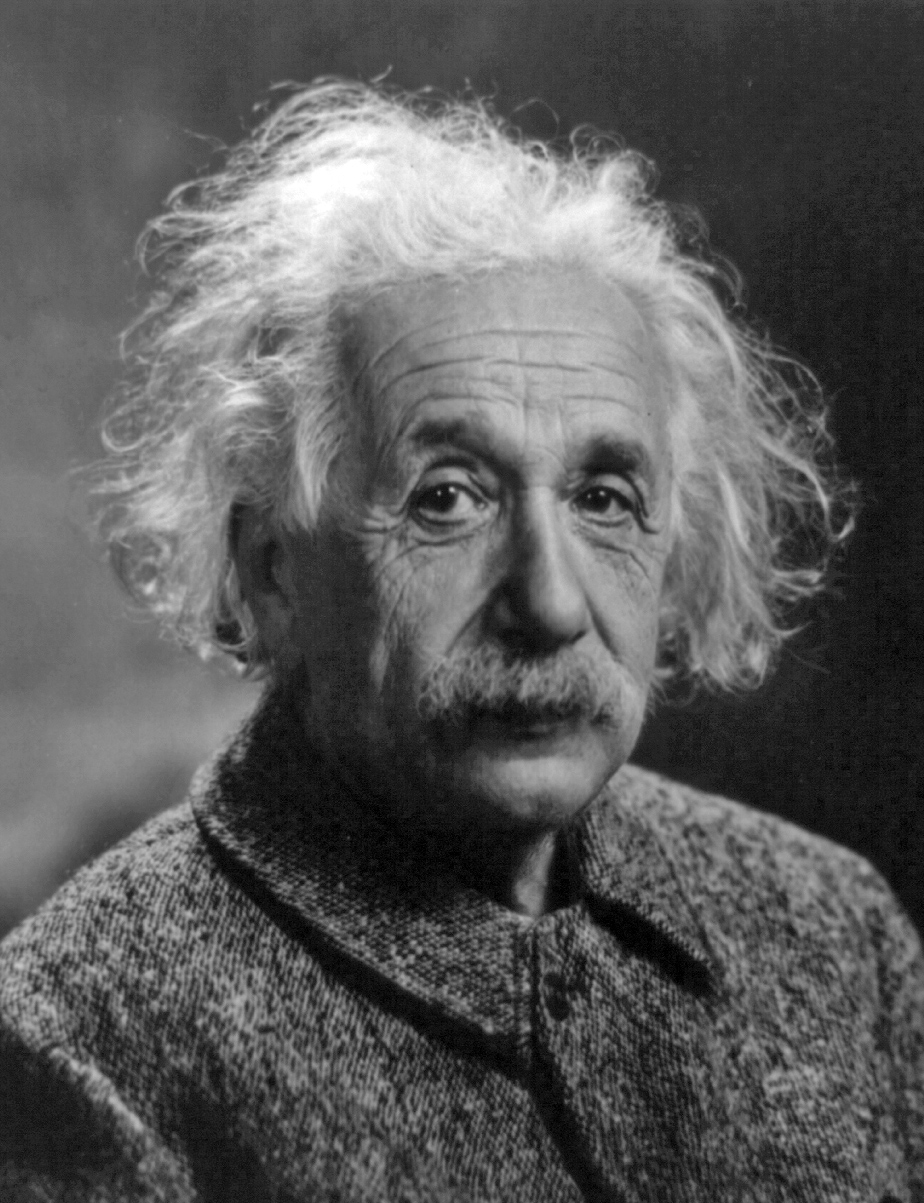
\includegraphics[height=35mm]{mypicture}}
%\newcommand{\Photo}{}

\begin{document}
\vspace*{4cm}
\title{Instructions for producing a camera-ready manuscript}


\author{ A.B. Author }

\address{Department of Physics, Theoretical Physics, 1 Keble Road,\\
Oxford OX1 3NP, England}

\maketitle\abstracts{
This is where the abstract should be placed. It should consist of one paragraph
and give a concise summary of the material in the article below.
Replace the title, authors, and addresses within the curly brackets
with your own title, authors, and addresses; please use
capital letters for the title and the authors. You may have as many authors and
addresses as you wish. It's preferable not to use footnotes in the abstract
or the title; the
acknowledgments for funding bodies etc. are placed in a separate section at
the end of the text.}

\section{Guidelines}

The Moriond proceedings are printed from camera-ready manuscripts.
The following guidelines are intended to get a uniform rending of the 
proceedings. Authors with no connection to \LaTeX{} should use this
sample text as a guide for their presentation using their favorite
text editor (see section~\ref{subsec:final})

\subsection{Producing the Hard Copy}\label{subsec:prod}

The hard copy may be printed using the procedure given below.
You should use
two files: \footnote{You can get these files from
our site at \url{http://moriond.in2p3.fr/2023/download/moriond.tar.gz}.}
\begin{description}
\item[\texttt{moriond.cls}] the style file that provides the higher
level \LaTeX{} commands for the proceedings. Don't change these parameters.
\item[\texttt{moriond.tex}] the main text. You can delete our sample
text and replace it with your own contribution to the volume, however we
recommend keeping an initial version of the file for reference.
\end{description}
The command for (pdf)\LaTeX ing is \texttt{pdflatex moriond}: do this twice to
sort out the cross-referencing.

%If there is an abbreviation
%defined in the new definitions at the top of the file {\em moriond.tex} that
%conflicts with one of your own macros, then
%delete the appropriate command and revert to longhand. Failing that, please
%consult your local texpert to check for other conflicting macros that may
%be unique to your computer system.
{\bf Page numbers should not appear.}

\subsection{Headings and Text and Equations}

Please preserve the style of the
headings, text fonts and line spacing to provide a
uniform style for the proceedings volume.

Equations should be centered and numbered consecutively, as in
Eq.~\ref{eq:murnf}, and the {\em eqnarray} environment may be used to
split equations into several lines, for example in Eq.~\ref{eq:sp},
or to align several equations.
An alternative method is given in Eq.~\ref{eq:spa} for long sets of
equations where only one referencing equation number is wanted.

In \LaTeX, it is simplest to give the equation a label, as in
Eq.~\ref{eq:murnf}
where we have used \verb^\label{eq:murnf}^ to identify the
equation. You can then use the reference \verb^\ref{eq:murnf}^
when citing the equation in the
text which will avoid the need to manually renumber equations due to
later changes. (Look at
the source file for some examples of this.)

The same method can be used for referring to sections and subsections.

\subsection{Tables}

The tables are designed to have a uniform style throughout the proceedings
volume. It doesn't matter how you choose to place the inner
lines of the table, but we would prefer the border lines to be of the style
shown in Table~\ref{tab:exp}.
 The top and bottom horizontal
lines should be single (using \verb^\hline^), and
there should be single vertical lines on the perimeter,
(using \verb^\begin{tabular}{|...|}^).
 For the inner lines of the table, it looks better if they are
kept to a minimum. We've chosen a more complicated example purely as
an illustration of what is possible.

The caption heading for a table should be placed at the top of the table.

\begin{table}[t]
\caption[]{Experimental Data bearing on $\Gamma(K \ra \pi \pi \gamma)$
for the $\ko_S, \ko_L$ and $K^-$ mesons.}
\label{tab:exp}
\vspace{0.4cm}
\begin{center}
\begin{tabular}{|c|c|c|l|}
\hline
& & & \\
&
$\Gamma(\pi^- \pi^0)\; s^{-1}$ &
$\Gamma(\pi^- \pi^0 \gamma)\; s^{-1}$ &
\\ \hline
\mco{2}{|c|}{Process for Decay} & & \\
\cline{1-2}
$K^-$ &
$1.711 \times 10^7$ &
\begin{minipage}{1in}
$2.22 \times 10^4$ \\ (DE $ 1.46 \times 10^3)$
\end{minipage} &
\begin{minipage}{1.5in}
No (IB)-E1 interference seen but data shows excess events relative to IB over
$E^{\ast}_{\gamma} = 80$ to $100MeV$
\end{minipage} \\
& & &  \\ \hline
\end{tabular}
\end{center}
\end{table}


\subsection{Figures}\label{subsec:fig}

If you wish to `embed' an image or photo in the file, you can use
the present template as an example. The command 
\verb^\includegraphics^ can take several options, like
\verb^draft^ (just for testing the positioning of the figure)
or \verb^angle^ to rotate a figure by a given angle.

The caption heading for a figure should be placed below the figure.

\subsection{Limitations on the Placement of Tables,
Equations and Figures}\label{sec:plac}

Very large figures and tables should be placed on a page by themselves. One
can use the instruction \verb^\begin{figure}[p]^ or
\verb^\begin{table}[p]^
to position these, and they will appear on a separate page devoted to
figures and tables. We would recommend making any necessary
adjustments to the layout of the figures and tables
only in the final draft. It is also simplest to sort out line and
page breaks in the last stages.

\subsection{Acknowledgments, Appendices, Footnotes and the Bibliography}

If you wish to have
acknowledgments to funding bodies etc., these may be placed in a separate
section at the end of the text, before the Appendices. This should not
be numbered so use \verb^\section*{Acknowledgments}^.

It's preferable to have no appendices in a brief article, but if more
than one is necessary then simply copy the
\verb^\section*{Appendix}^
heading and type in Appendix A, Appendix B etc. between the brackets.

Footnotes are denoted by a letter superscript
in the text,\footnote{Just like this one.} and references
are denoted by a number superscript.

Bibliography can be generated either manually or through the BibTeX
package (which is recommanded). In this sample we
have used \verb^\bibitem^ to produce the bibliography.
Citations in the text use the labels defined in the bibitem declaration,
for example, the first paper by Jarlskog~\cite{ja} is cited using the command
\verb^\cite{ja}^.

%If you more commonly use the method of square brackets in the line of text
%for citation than the superscript method,
%please note that you need  to adjust the punctuation
%so that the citation command appears after the punctuation mark.

\subsection{Photograph}

You may want to include a photograph of yourself below the title
of your talk. A scanned photo can be 
directly included using the default command\\
\verb^\newcommand{\Photo}{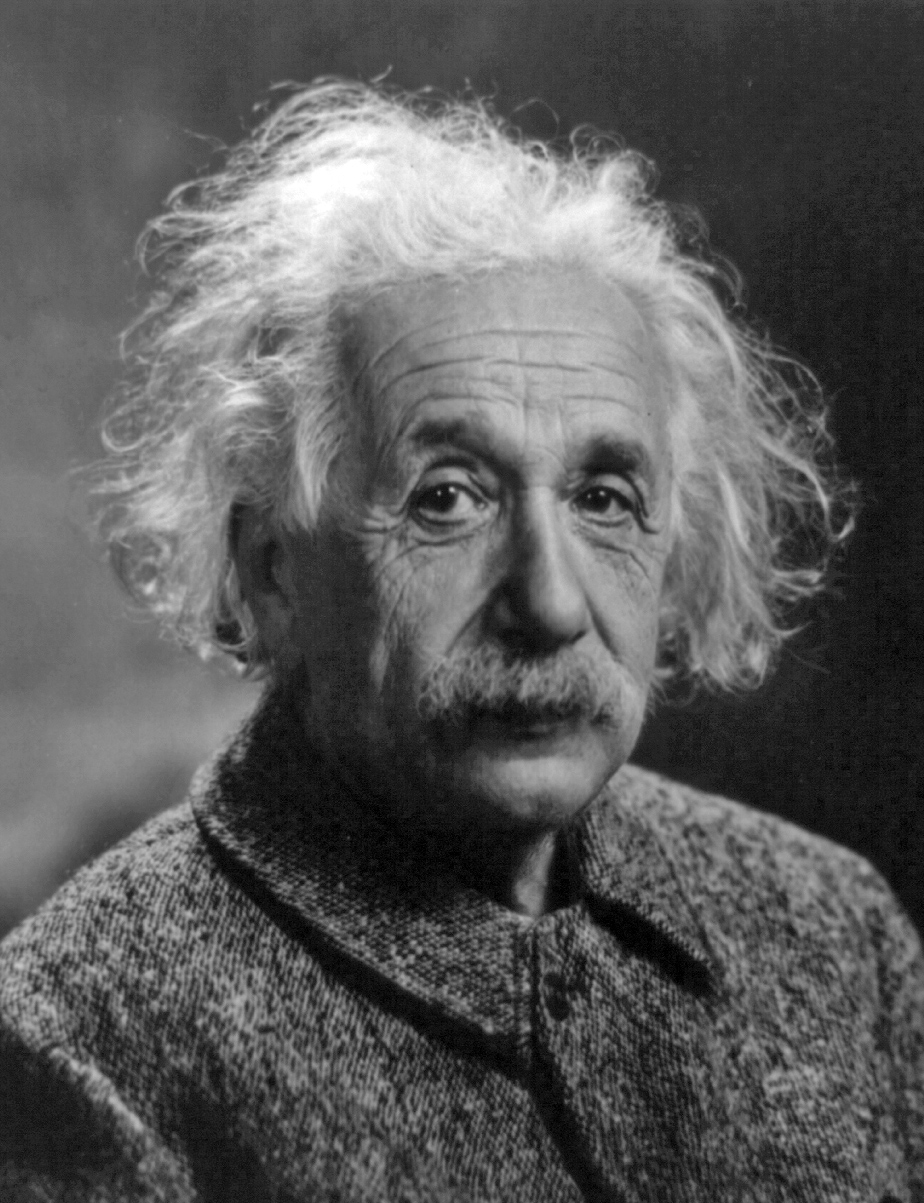
\includegraphics[height=35mm]{mypicture}}^\\
just before the 
\verb^\begin{document}^
line. If you don't want to include your photo, just comment this line
by adding the \verb^%^ sign at the beginning of 
the line and uncomment the next one
\verb^%\newcommand{\Photo}{}^ by removing its \verb^%^ sign.

\subsection{Final Manuscript}\label{subsec:final}

All files (.tex, figures and .pdf) should be sent by the {\bf 15th of May 2023}
by e-mail 
to \\
{\bf moriond@in2p3.fr}.\\

\section{Sample Text }

The following may be (and has been) described as `dangerously irrelevant'
physics. The Lorentz-invariant phase space integral for
a general n-body decay from a particle with momentum $P$
and mass $M$ is given by:
\begin{equation}
I((P - k_i)^2, m^2_i, M) = \frac{1}{(2 \pi)^5}\!
\int\!\frac{d^3 k_i}{2 \omega_i} \! \delta^4(P - k_i).
\label{eq:murnf}
\end{equation}
The only experiment on $K^{\pm} \ra \pi^{\pm} \pi^0 \gamma$ since 1976
is that of Bolotov {\it et al}.~\cite{bu}
        There are two
necessary conditions required for any acceptable
parametrization of the
quark mixing matrix. The first is that the matrix must be unitary, and the
second is that it should contain a CP violating phase $\delta$.
 In Sec.~\ref{subsec:fig} the connection between invariants (of
form similar to J) and unitarity relations
will be examined further for the more general $ n \times n $ case.
The reason is that such a matrix is not a faithful representation of the group,
i.e. it does not cover all of the parameter space available.
\begin{equation}
\renewcommand{\arraystretch}{1.2}
\begin{array}{rc@{\,}c@{\,}l}
%\begin{array}{>{\displaystyle}r>{\displaystyle}c>{\displaystyle}c>{\displaystyle}l}

%\begin{eqnarray}
\bf{K} & = &&  Im[V_{j, \alpha} {V_{j,\alpha + 1}}^*
{V_{j + 1,\alpha }}^* V_{j + 1, \alpha + 1} ] \\
       &   & + & Im[V_{k, \alpha + 2} {V_{k,\alpha + 3}}^*
{V_{k + 1,\alpha + 2 }}^* V_{k + 1, \alpha + 3} ]  \\
       &   & + & Im[V_{j + 2, \beta} {V_{j + 2,\beta + 1}}^*
{V_{j + 3,\beta }}^* V_{j + 3, \beta + 1} ]  \\
       &   & + & Im[V_{k + 2, \beta + 2} {V_{k + 2,\beta + 3}}^*
{V_{k + 3,\beta + 2 }}^* V_{k + 3, \beta + 3}] \\
& & \\
\bf{M} & = &&  Im[{V_{j, \alpha}}^* V_{j,\alpha + 1}
V_{j + 1,\alpha } {V_{j + 1, \alpha + 1}}^* ]  \\
       &   & + & Im[V_{k, \alpha + 2} {V_{k,\alpha + 3}}^*
{V_{k + 1,\alpha + 2 }}^* V_{k + 1, \alpha + 3} ]  \\
       &   & + & Im[{V_{j + 2, \beta}}^* V_{j + 2,\beta + 1}
V_{j + 3,\beta } {V_{j + 3, \beta + 1}}^* ]  \\
       &   & + & Im[V_{k + 2, \beta + 2} {V_{k + 2,\beta + 3}}^*
{V_{k + 3,\beta + 2 }}^* V_{k + 3, \beta + 3}],
\\ & &
\end{array}
%\end{eqnarray}
\label{eq:spa}
\end{equation}

where $ k = j$ or $j+1$ and $\beta = \alpha$ or $\alpha+1$, but if
$k = j + 1$, then $\beta \neq \alpha + 1$ and similarly, if
$\beta = \alpha + 1$ then $ k \neq j + 1$.\footnote{An example of a
matrix which has elements
containing the phase variable $e^{i \delta}$ to second order, i.e.
elements with a
phase variable $e^{2i \delta}$ is given at the end of this section.}
   There are only 162 quark mixing matrices using these parameters
which are
to first order in the phase variable $e^{i \delta}$ as is the case for
the Jarlskog parametrizations, and for which J is not identically
zero.
It should be noted that these are physically identical and
form just one true parametrization.
\bea
T & = & Im[V_{11} {V_{12}}^* {V_{21}}^* V_{22}]  \nonumber \\
&  & + Im[V_{12} {V_{13}}^* {V_{22}}^* V_{23}]   \nonumber \\
&  & - Im[V_{33} {V_{31}}^* {V_{13}}^* V_{11}].
\label{eq:sp}
\eea


\begin{figure}
\begin{minipage}{0.33\linewidth}
\centerline{
\includegraphics[width=0.7\linewidth,draft=true]{figexamp}}
\end{minipage}
\hfill
\begin{minipage}{0.32\linewidth}
\centerline{
\includegraphics[width=0.7\linewidth]{figexamp}}
\end{minipage}
\hfill
\begin{minipage}{0.32\linewidth}
\centerline{
\includegraphics[angle=-45,width=0.7\linewidth]{figexamp}}
\end{minipage}
\caption[]{same figure with draft option (left), normal (center) and rotated (right)}
\label{fig:radish}
\end{figure}

\section*{Acknowledgments}

This is where one places acknowledgments for funding bodies etc.
Note that there are no section numbers for the Acknowledgments, Appendix
or References.

\section*{Appendix}

 We can insert an appendix here and place equations so that they are
given numbers such as Eq.~\ref{eq:app}.
\be
x = y.
\label{eq:app}
\ee

\section*{References}

\begin{thebibliography}{99}
\bibitem{ja}C Jarlskog in {\em CP Violation}, ed. C Jarlskog
(World Scientific, Singapore, 1988).

\bibitem{ma}L. Maiani, \Journal{\PLB}{62}{183}{1976}.

\bibitem{bu}J.D. Bjorken and I. Dunietz, \Journal{\PRD}{36}{2109}{1987}.

\bibitem{bd}C.D. Buchanan {\it et al}, \Journal{\PRD}{45}{4088}{1992}.

\end{thebibliography}

\end{document}

%%%%%%%%%%%%%%%%%%%%%%
% End of moriond.tex  %
%%%%%%%%%%%%%%%%%%%%%%


%%% Local Variables: 
%%% mode: latex
%%% TeX-master: t
%%% End: 

%%% Local Variables: 
%%% mode: latex
%%% TeX-master: t
%%% End: 

%%% Local Variables: 
%%% mode: latex
%%% TeX-master: t
%%% End: 
